\noindent\textbf{Problem 1:} (i) Apply available expression analysis to the following
CFG to find the AvailIn set for each BB ; (ii) Based on the results of available
expression analysis, use GCSE (Global Common Subexpression Elimination) to find out
the redundant computations and remove them.

\newcolumntype{M}[1]{>{\centering\arraybackslash}m{#1}}
\newcolumntype{N}{@{}m{0pt}@{}}

\begin{center}
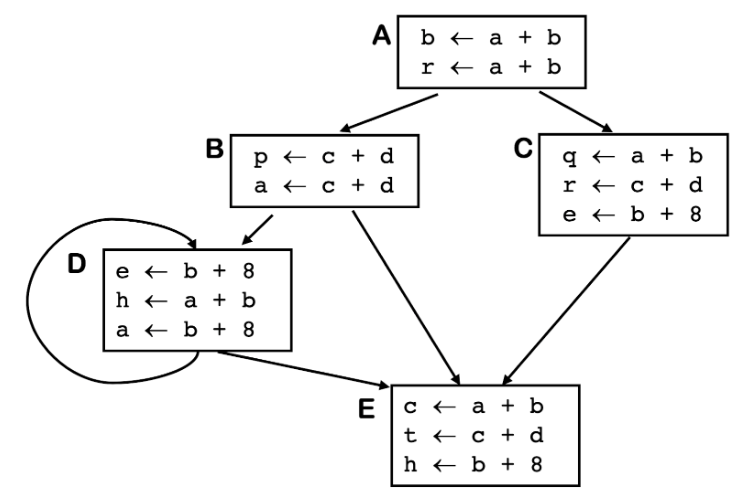
\includegraphics[scale=0.5]{prob1.png}
\end{center}

\noindent
{\renewcommand{\arraystretch}{2}
\begin{tabularx}{\textwidth}{|X|X|X|X|X|X|}
\hline
Block & A & B & C & D & E \\
\hline
Block & A & B & C & D & E \\ [1em]
\hline
\end{tabularx}
}

\vskip 0.1in

\noindent \textit{Tips: to apply GCSE, you can first find the redundant computations
(expressions), then create the global hash names only for those expressions,
and finally, transform the CFG to remove the redundancies.}